%%%%%
% 
\documentclass[mathserif,graphics]{beamer}
\usepackage{Sweave}
\mode<presentation>
\usetheme{Boadilla} % Beamer Theme
\usecolortheme{whale}
\usepackage{amsmath} % for math AMS fonts
\usepackage{centernot}
\usepackage{graphicx} % to include figures
\usepackage{subfigure} % to have figures in figures
\usepackage{multimedia} % to include movies

\usepackage[utf8]{inputenc}
\usepackage{amsfonts}
\usepackage{natbib}
\usepackage{scrpage2}
\usepackage{dsfont}
\usepackage{float}
\usepackage{amssymb}

\usepackage{bbm}

\usepackage{tikz}
\usetikzlibrary{arrows,shapes,backgrounds, patterns, decorations.markings} % loads some tikz extensions
\usepackage[english]{babel}
\useoutertheme[subsection=false]{smoothbars} % Beamer Outer Theme
\usepackage{mdframed}
\usepackage{boxedminipage}
\newcommand{\hlcolor}[2]{{\setlength{\fboxsep}{0pt}\colorbox{#1}{\strut #2}}}
\newcommand{\eg}{e.\,g. }
\newcommand{\ie}{i.\,e. }
\newcommand{\cdf}{c.\,d.\,f. }
%\usepackage[usenames,dvipsnames]{xcolor}
\definecolor{lightblue}{rgb}{0.8,0.85,1}


\defbeamertemplate*{footline}{my infolines theme}
    {
      \leavevmode%
      \hbox{%
      \begin{beamercolorbox}[wd=.44\paperwidth,ht=2.25ex,dp=1ex,center]{author
      in head/foot}%
        \usebeamerfont{author in head/foot}\insertshortauthor~~\insertshortinstitute
      \end{beamercolorbox}%
      \begin{beamercolorbox}[wd=.2\paperwidth,ht=2.25ex,dp=1ex,center]{title in
      head/foot}%
        \usebeamerfont{title in head/foot}\insertshorttitle
      \end{beamercolorbox}%
      \begin{beamercolorbox}[wd=.36\paperwidth,ht=2.25ex,dp=1ex,right]{date in
      head/foot}%
        \usebeamerfont{date in head/foot}\insertshortdate{}\hspace*{2em}
        \insertframenumber{} / \inserttotalframenumber\hspace*{2ex}
      \end{beamercolorbox}}%
      \vskip0pt%
    }

\title{Normal Distribution}
%\subtitle{Seminar graph algorithms}
\author{Andrey Chinnov, Sebastian Honermann, Carlos Zydorek}
%\institute{Seminar graph algorithms}
\date{Case Studies \\
"Data Analytics"}

\begin{document}
\frame{
\titlepage
\setbeamercovered{dynamic}
}



\section{Introduction}
\frame{
\frametitle{Outline}
\begin{enumerate}
\item \alert {Introduction}
  \begin{itemize}
  \item Normality as a requirement for statistical methods
  \item Data Set Overview
  \end{itemize}
\item Normality Testing
  \begin{itemize}
  \item Graphical Methods for Normality Testing
    \begin{itemize}
    \item Q-Q-Plots
    \item Chi-Square Plot
    \end{itemize}
  \item Quantitative Methods for Normality Testing
    \begin{itemize}
    \item Shapiro-Wilk Test
    \item Pearson's Chi-Squared Test
    \item Kolmogorov-Smirnov Test
    \end{itemize}
  \end{itemize}
\item Transformation to Normality
  \begin{itemize}
  \item Box-Cox Transformation
  \item Transformation Results Testing 
  \end{itemize}
\item Summary
\end{enumerate}
}
\subsection{Normality as a requirement for statistical methods}

\frame{
\frametitle{Normality as a requirement for statistical methods}

}

\subsection{Data Set Overview}

\frame{
\frametitle{Data Set Overview}

}

\section{Normality Testing}
\frame{
\frametitle{Outline}
\begin{enumerate}
\item Introduction
  \begin{itemize}
  \item Normality as a requirement for statistical methods
  \item Data Set Overview
  \end{itemize}
\item \alert{Normality Testing}
  \begin{itemize}
  \item Graphical Methods for Normality Testing
    \begin{itemize}
    \item Q-Q-Plots
    \item Chi-Square Plot
    \end{itemize}
  \item Quantitative Methods for Normality Testing
    \begin{itemize}
    \item Shapiro-Wilk Test
    \item Pearson's Chi-Squared Test
    \item Kolmogorov-Smirnov Test
    \end{itemize}
  \end{itemize}
\item Transformation to Normality
  \begin{itemize}
  \item Box-Cox Transformation
  \item Transformation Results Testing 
  \end{itemize}
\item Summary
\end{enumerate}
}

\subsection{Q-Q-Plots}
\frame{
\frametitle{Graphical Methods for Normality Testing}
\framesubtitle{Q-Q-Plots}
}

\subsection{Chi-Square Plot}
\frame{
\frametitle{Graphical Methods for Normality Testing}
\framesubtitle{Chi-Square Plot}
}

\subsection{Shapiro-Wilk Test}
\frame{
\frametitle{Quantitative Methods for Normality Testing}
\framesubtitle{Shapiro-Wilk Test}
}

\subsection{Pearson's Chi-Squared Test}
\frame{
\frametitle{Quantitative Methods for Normality Testing}
\framesubtitle{Pearson's Chi-Squared Test}
}

\subsection{Kolmogorov-Smirnov Test}
\frame{
\frametitle{Quantitative Methods for Normality Testing}
\framesubtitle{Kolmogorov-Smirnov Test}
Let $x=(x_1,x_2, \dots, x_n)$ be a sample of unknown
distribution $\mathbb{P}$.
\begin{columns}[t]
\column{0.5\columnwidth}
\begin{definition}
$F_n(x)=\frac{1}{n}\sum_{i=1}^n \mathbbm{1}_{\{x_i\le x\}}(x)$ \\
- \alert{empirical} \cdf, where \\
$\mathbbm{1}_{\{x_i\le x\}}(x)=\left\lbrace 
\begin{array}{cll}
                1 & \mbox{if} \ x_i\le x\\
                 0 & \mbox{otherwise}.
\end{array} 
\right.$
\end{definition}
\onslide<2->{
$F(x)$ - theoretical normal \cdf with
\[\bar{x}=\frac{1}{n}\sum_i x_i,\quad \sigma^2_x=\frac{1}{n}(x_i-\bar{x})^2\]}
\onslide<3->{
$d=\sup_{x\in \mathbb{R}}|F_n(x)-F(x)|$ \\- distance between them.}
\column{0.5\columnwidth}
  \vspace{-1cm}
    \only<1>{
    \begin{figure}
	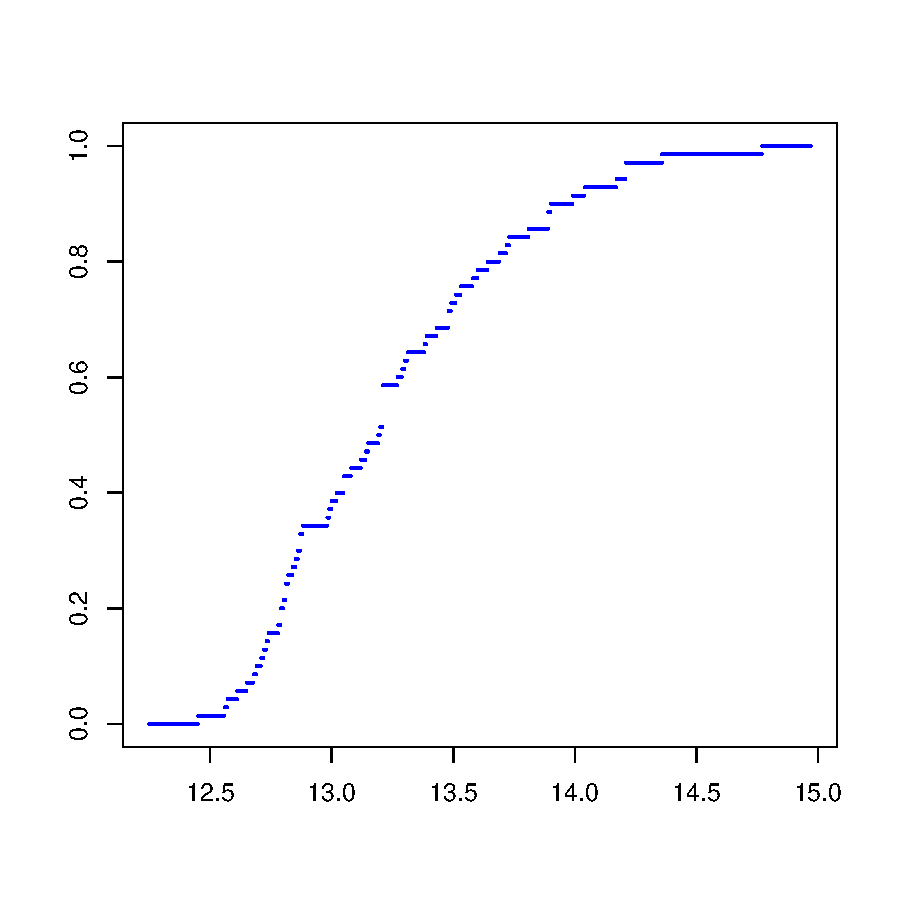
\includegraphics[width=\columnwidth]{Report-empiricFunc}
	\end{figure}}
    \only<2->{
    \begin{figure}
	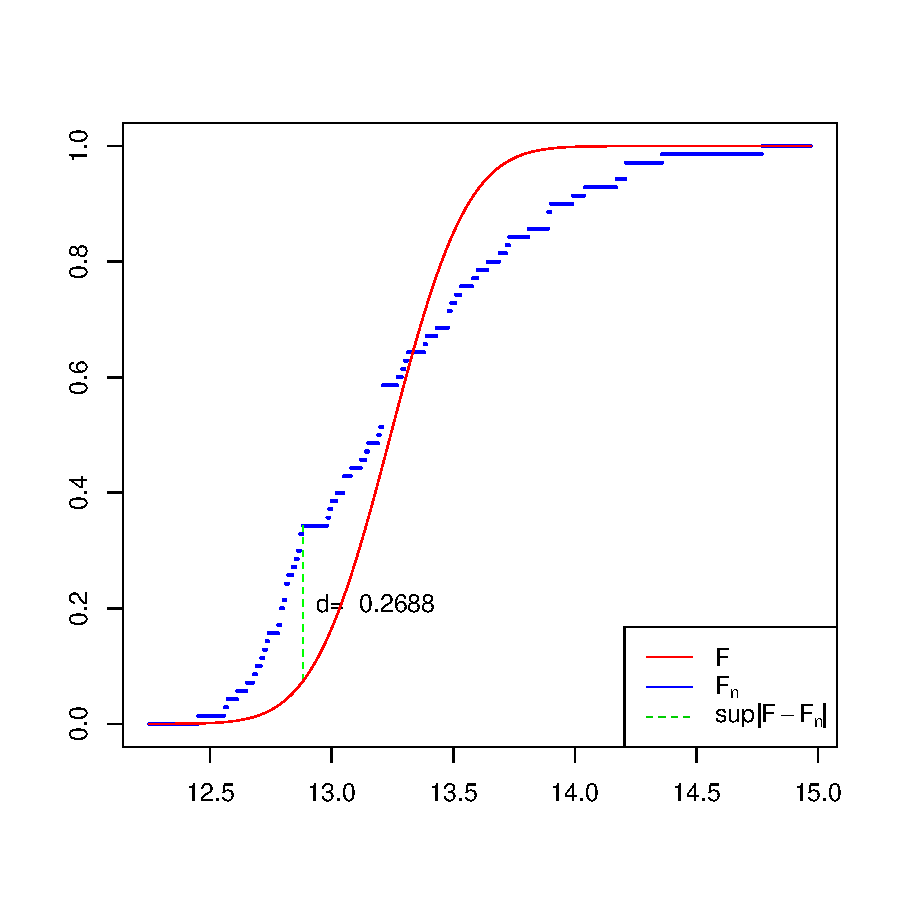
\includegraphics[width=\columnwidth]{Report-empiricTeorFunc}
	\end{figure}}
\vspace{-1.5cm}
\begin{center}
Glass Type 1, Natrium (Na)
\end{center}
\end{columns}
}

\frame{
\frametitle{Quantitative Methods for Normality Testing}
\framesubtitle{Kolmogorov-Smirnov Test}
Let $x=(x_1,x_2, \dots, x_n)$ be a sample of unknown
distribution $\mathbb{P}$.\\
Theoretical \cdf $F$ defines a distribution $\mathbb{P}_0$.\\
\onslide<2->{
\[\begin{array}{rcl}
H_0 & : & \mathbb{P} = \mathbb{P}_0,\\
H_1 & : & \mathbb{P} \ne \mathbb{P}_0.
\end{array}\]}
\onslide<3->{
KS test statistics:
\[D_n = \sqrt{n}\cdot \sup_{x \in \mathbb{R}}|F_n(x)-F(x)|.\]}
\onslide<4->{
Properties of $D_n$ in case $H_0$ is \alert{TRUE}:}
\begin{itemize}
\item<4-> Distribution of $\hat{D}_n:=(D_1,D_2,\dots, D_n)$ does not depend on
$F$\\
\onslide<5->{\hfill$\implies$ \alert{tabulated}}
\item<6-> $\forall t>0:$ \[P(D_n\le t)\xrightarrow[n \to \infty]{}
H(t)=1-2\sum_{i=1}^{\infty}(-1)^{i-1} \exp^{-2i^2t^2}\]
\end{itemize}

\vspace{15cm}
}

\frame{
\frametitle{Quantitative Methods for Normality Testing}
\framesubtitle{Kolmogorov-Smirnov Test}
The KS test uses the decision rule
\[ \delta = 
\left\{
\begin{array}{rcl}
H_0&:& D_n\le c\\
H_1&:& D_n> c
\end{array}
\right.,
\]
where $c$ - critical value \onslide<2-> {that\\
depends on a significance level $\alpha$:}
\[\onslide<3->{\alpha = P(\delta \ne H_0|H_0)}\onslide<4->{=P(D_n>c|H_0)}\onslide<5->{=1-P(D_n\le c|H_0)}\onslide<6->{\approx 1-H(c).}\]
\onslide<7->{\[\implies \alert{c\approx H_{1-\alpha}}\]}

\vspace{15cm}
}

\frame{
\frametitle{Quantitative Methods for Normality Testing}
\framesubtitle{Kolmogorov-Smirnov Test}
The KS test uses the decision rule for a given significance level $\alpha$
\[ \delta = 
\left\{
\begin{array}{rcl}
H_0&:& D_n\le H_{1-\alpha}\\
H_1&:& D_n> H_{1-\alpha}
\end{array}
\right., \quad H(t)=1-2\sum_{i=1}^{\infty}(-1)^{i-1} \exp^{-2i^2t^2}
\]
\begin{columns}[t]
\column{0.5\columnwidth}
\onslide<2->{\centerline{{\bf Example:}}}\\
\begin{itemize}
\item<3->
$n=70$
\item<4->
$D_n=\sqrt{n}
\sup|F_n-F|=2.2493$
\item<5->
$\alpha = 0.01$\\
\hfill$\implies
c=H_{1-\alpha}=1.6276$

\item<6->
$D_n>c \implies  H_0$ \alert{rejected}

\item<7-> 
$\implies \mathbb{P}\ne \mathbb{P}_0$

\item<8-> \alert{$\centernot\implies$
 data not normally distributed!!!}
\end{itemize}

\column{0.5\columnwidth}
  \vspace{-1.9cm}
    \onslide<2->{
    \begin{figure}
	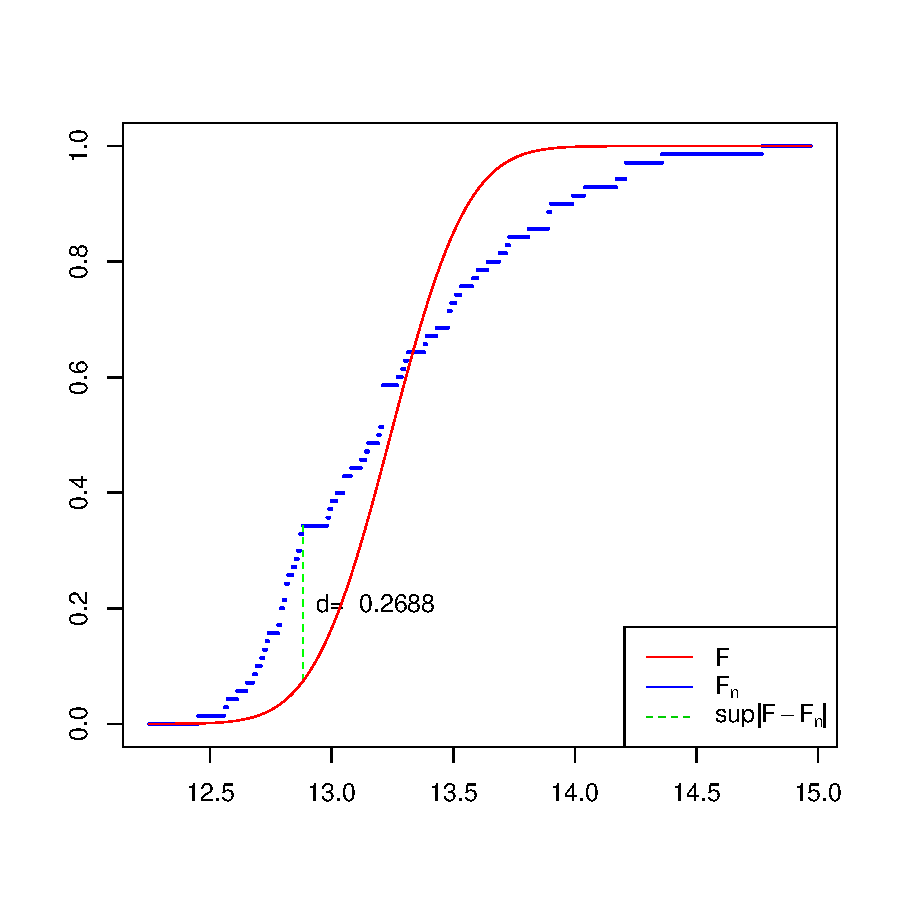
\includegraphics[width=\columnwidth]{Report-empiricTeorFunc}
	\end{figure}
\vspace{-1.5cm}
\begin{center}
Glass Type 1, Natrium (Na)
\end{center}}
\end{columns}

\vspace{15cm}
}

\begin{frame}[fragile]
\frametitle{Quantitative Methods for Normality Testing}
\framesubtitle{Improved Kolmogorov-Smirnov Test}
KS test is improved by solving the following
optimization problem \[KS(\mu,\sigma)=\sup_{x \in
\mathbb{R}}|F_n(x)-F(x,\mu,\sigma)|\to \min.\]
\begin{itemize}
\item<1->[]$R$ code used:
\item<2->[]
\begin{Schunk}
\begin{Sinput}
 c(mean(dat),var(dat))
\end{Sinput}
\begin{Soutput}
[1] 13.2422857  0.2493019
\end{Soutput}
\begin{Sinput}
 #optim is a predifined R function in stats package
 #defalut method of optimization is Nelder and Mead
 result = optim(c(mean(dat),var(dat)),KS)
 result$par
\end{Sinput}
\begin{Soutput}
[1] 13.1769501  0.4682486
\end{Soutput}
\begin{Sinput}
 result$value
\end{Sinput}
\begin{Soutput}
[1] 0.07870673
\end{Soutput}
\end{Schunk}
\end{itemize}
\vspace{10cm}
\end{frame}


\frame{
\frametitle{Quantitative Methods for Normality Testing}
\framesubtitle{Improved Kolmogorov-Smirnov Test}
KS test is improved by solving the following
optimization problem \[KS(\mu,\sigma)=\sup_{x \in
\mathbb{R}}|F_n(x)-F(x,\mu,\sigma)|\to \min.\]
\begin{columns}[t]
\column{0.5\columnwidth}
\vspace{-1cm}
\begin{itemize}
\item<1->Initial vector of parameters
$\mu=13.2423,\quad
\sigma^2=0.2493$
\item<1->Optimized vector of parameters
$\hat{\mu}=13.1770, \quad
\hat{\sigma}^2=0.4682$
\item<3->
$D_n=\sqrt{n}
\sup|F_n-F_{new}|=0.6585$
\item<4->
$c=1.6276$
\item<5->
$D_n<c \implies  H_0$ \alert{accepted}

\item<6-> 
$\implies \mathbb{P}= \mathbb{P}_0$

\item<7-> \alert{$\implies$
 data normally distributed!}
\end{itemize}

\column{0.5\columnwidth}
  \vspace{-1.9cm}
    \only<1>{
    \begin{figure}
	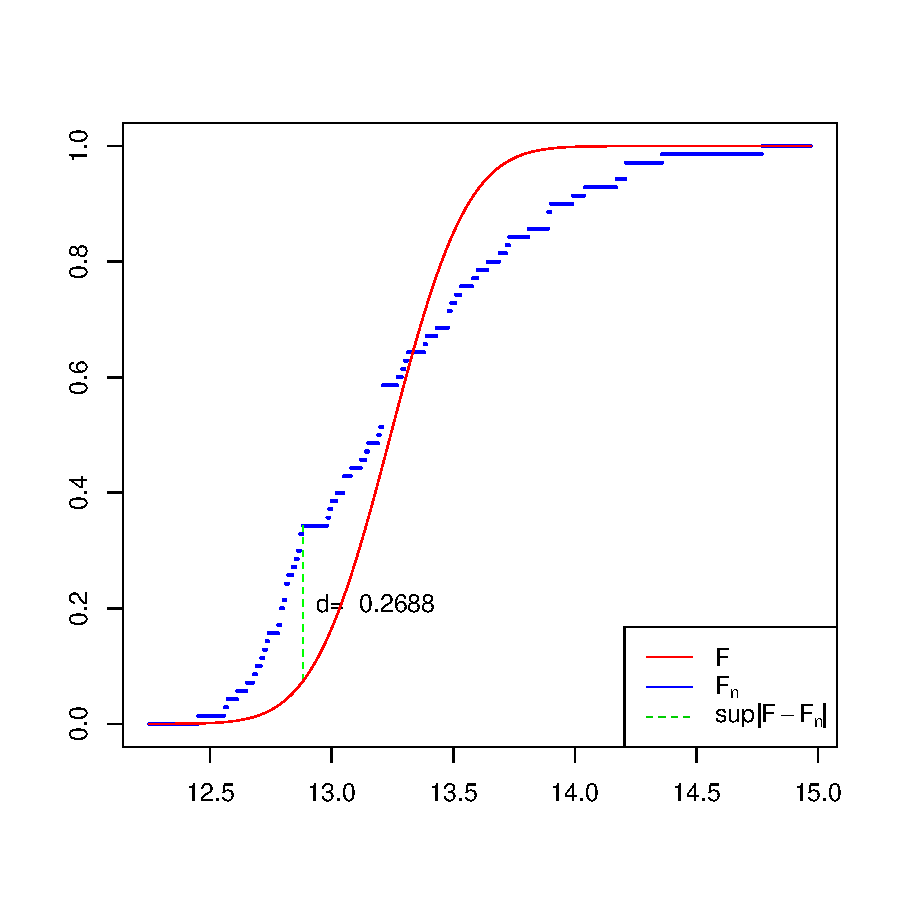
\includegraphics[width=\columnwidth]{Report-empiricTeorFunc}
	\end{figure}}
    \only<2->{
    \begin{figure}
	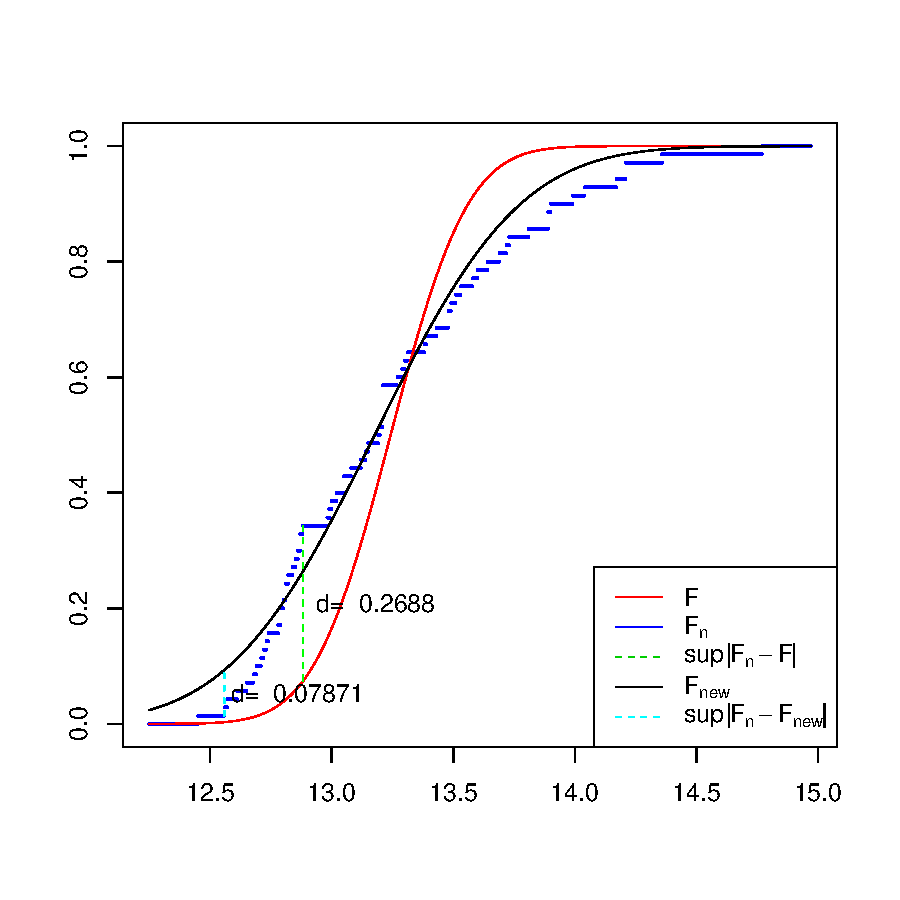
\includegraphics[width=\columnwidth]{Report-improvedKS}
	\end{figure}}
\onslide<2->{
\vspace{-1.5cm}
\begin{center}
Glass Type 1, Natrium (Na)
\end{center}}
\end{columns}

\vspace{15cm}
}


\frame{
\frametitle{Quantitative Methods for Normality Testing}
\framesubtitle{Improved Kolmogorov-Smirnov Test Results}
Results of Improved KS test on the whole data set:
\only<1>{
\scriptsize
\begin{table}[h!]
\centering
\begin{tabular}{|cccccc|} \hline variable & test statistic & sig. level & critical value & p-value & rejected\\ \hline RI & 1.34 & 0.01 & 1.63 & 0.0561963016778131 & no\\ 
Na & 0.87 & 0.01 & 1.63 & 0.43825271603342 & no\\ 
Mg & 2.94 & 0.01 & 1.63 & 6.18457917100912e-08 & yes\\ 
Al & 0.84 & 0.01 & 1.63 & 0.474757887353829 & no\\ 
Si & 0.96 & 0.01 & 1.63 & 0.314710019077325 & no\\ 
K & 2.14 & 0.01 & 1.63 & 0.000212776619708754 & yes\\ 
Ca & 1.33 & 0.01 & 1.63 & 0.057710602872685 & no\\ 
Ba & 2.60 & 0.01 & 1.63 & 2.75476085742632e-06 & yes\\ 
Fe & 4.68 & 0.01 & 1.63 & < 1.0e-15 & yes\\ \hline \end{tabular}
\label{tab:KS-full}
\end{table}}
\only<2>{
\scriptsize
\begin{columns}[t]
\column{0.3\columnwidth}
\begin{table}[h!]
\centering
\begin{tabular}{|cc|} \hline variable & rejected\\ 
\hline RI & no\\ 
Na & no\\ 
Mg & yes\\ 
Al & no\\ 
Si & no\\ 
K & yes\\ 
Ca & no\\ 
Ba & yes\\ 
Fe & yes\\ \hline \end{tabular}
\end{table}}
\column{0.7\columnwidth}
\begin{figure}
	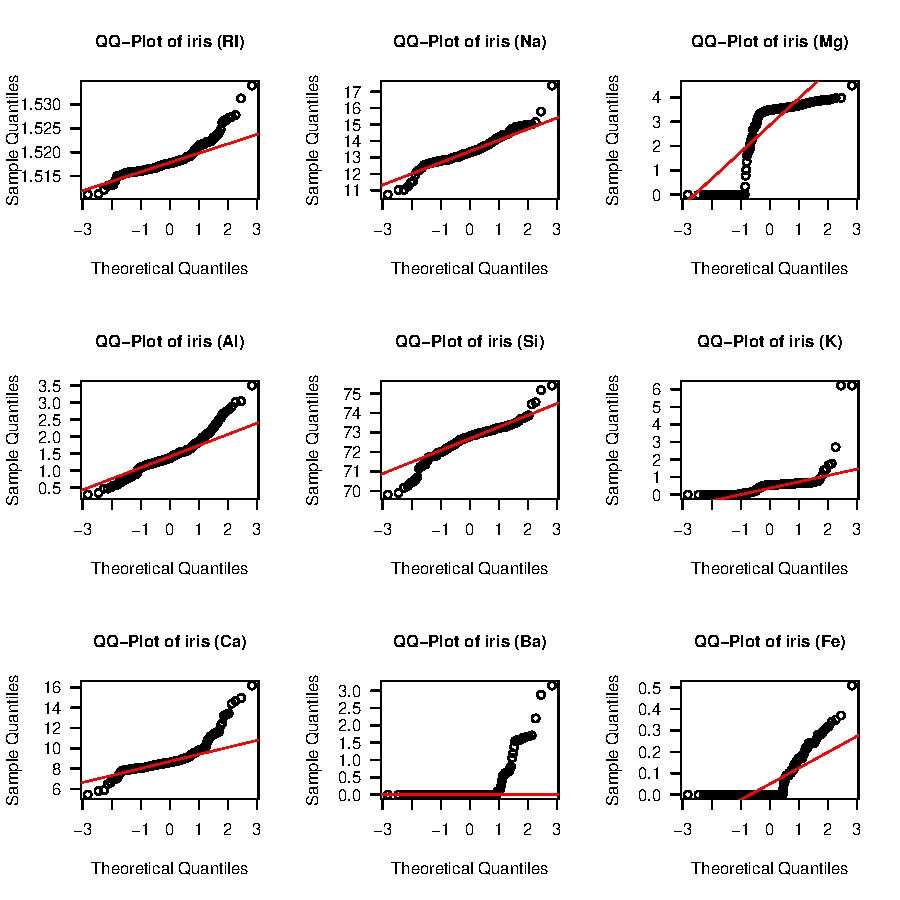
\includegraphics[width=\columnwidth]{auxiliary-drawQQPlots}
	\end{figure}
\end{columns}}
\vspace{15cm}
}

\section{Transformation to Normality}
\frame{
\frametitle{Outline}
\begin{enumerate}
\item Introduction
  \begin{itemize}
  \item Normality as a requirement for statistical methods
  \item Data Set Overview
  \end{itemize}
\item Normality Testing
  \begin{itemize}
  \item Graphical Methods for Normality Testing
    \begin{itemize}
    \item Q-Q-Plots
    \item Chi-Square Plot
    \end{itemize}
  \item Quantitative Methods for Normality Testing
    \begin{itemize}
    \item Shapiro-Wilk Test
    \item Pearson's Chi-Squared Test
    \item Kolmogorov-Smirnov Test
    \end{itemize}
  \end{itemize}
\item \alert{Transformation to Normality}
  \begin{itemize}
  \item Box-Cox Transformation
  \item Transformation Results Testing 
  \end{itemize}
\item Summary
\end{enumerate}
}
\subsection{Box-Cox Transformation}

\frame{
\frametitle{Box-Cox Transformation}

}

\subsection{Transformation Results Testing}

\frame{
\frametitle{Transformation Results Testing}

}

\section{Summary}
\frame{
\frametitle{Outline}
\begin{enumerate}
\item Introduction
  \begin{itemize}
  \item Normality as a requirement for statistical methods
  \item Data Set Overview
  \end{itemize}
\item Normality Testing
  \begin{itemize}
  \item Graphical Methods for Normality Testing
    \begin{itemize}
    \item Q-Q-Plots
    \item Chi-Square Plot
    \end{itemize}
  \item Quantitative Methods for Normality Testing
    \begin{itemize}
    \item Shapiro-Wilk Test
    \item Pearson's Chi-Squared Test
    \item Kolmogorov-Smirnov Test
    \end{itemize}
  \end{itemize}
\item Transformation to Normality
  \begin{itemize}
  \item Box-Cox Transformation
  \item Transformation Results Testing 
  \end{itemize}
\item \alert{Summary}
\end{enumerate}
}
\subsection{Summary}
\frame{
\frametitle{Summary}
}

\end{document}
